In this section, we analyze in the context of linear ridge regression how the dimension and precision of uniformly quantized word embeddings jointly impact generalization performance.
Though linear regression is evidently a very simplified setting, we believe the analysis in this setting is an important first step toward understanding the way compression affects generalization performance on downstream tasks.
We present two main results:
First, we show there is a bias-variance trade-off when choosing the embedding dimension, and that there can thus be an optimal dimension.
We then show that quantized embeddings can attain comparable generalization performance to full-precision embeddings at high compression rates when the spectrum of the embedding matrix decays slowly (which we empirically observe to be true).
Combined, these two results imply that one can attain large improvements in generalization performance in the memory constrained setting by using low-precision embeddings whose dimension approaches but does not exceed the optimal dimension.

%In this section, we present generalization bounds for linear regression models trained on top of uniformly quantized word embeddings.
%Though linear regression is evidently a very simplified setting, we believe the analysis in this setting is an important first step toward understanding the way compression affects generalization performance on downstream tasks.
%We present two main results:
%First, we show that when the standard deviation of the quantization noise is small relative to the regularization parameter $\lambda$ used to train the linear model, we attain good generalization bounds for the quantized embeddings relative to the full-precision embeddings.
%Second, we show that if the singular values of the embedding matrix decay slowly, then training the regression model with a large regularization parameter $\lambda$ cannot perform much worse than training with a smaller one.
%Combining these two results with our empirical observation that word embedding spectra decay relatively slowly helps explain why quantized word embeddings perform so well at high compression rates.

This section is organized as follows:
In Section~\ref{sec:background} we review fixed design linear ridge regression and discuss the trade-off involved in choosing the embedding dimension.
In Section~\ref{sec:theory_quantization} we present our analysis on the impact of quantization on generalization performance.

\subsection{Background: Generalization Bounds for Fixed Design Linear Regression}
\label{sec:background}
In fixed design linear regression, one is given a dataset $\{(x_i,y_i)\}_{i=1}^n$, for $x_i \in \RR^d$ and $y_i = \by_i + \eps_i \in \RR$, where the $\eps_i$ are independent random perturbations of the ``true labels'' $\by_i$ satisfying $\expect{}{\eps_i} = 0$ and $\var{}{\eps_i} = \sigma^2 < \infty$.
The goal is to design a training algorithm which takes as input the noisy dataset $\{(x_i,y_i)\}_{i=1}^n$ and outputs a model $f(x) = w^T x$ for which $\expect{}{\frac{1}{n}\sum_i (f(x_i) -\by_i)^2} \eqdef \cR(f)$ is small.
Linear ridge regression selects $w^* = \argmin_w \sum_i (w^T x_i - y_i)^2 + \lambda\|w\|_2^2$.
Letting $X \in \RR^{n\times d}$ be the matrix whose rows are $x_i$, $y \defeq (y_1,...,y_n) \in \RR^d$, and $I_d$ be the $d$-dimensional identity matrix, the minimizer of this optimization problem is $w^* = ( X^T X + \lambda I_d)^{-1}X^Ty$.
It is easy to show \citep{alaoui15} that the expected generalization error for the model $f_X(x) \defeq w^{*T}x$ is
\begin{eqnarray*}
\cR(f_X) &=& \frac{\lambda^2}{n} \by^T(XX^T + \lambda I_n)^{-2}\by \; +\\ && \frac{\sigma^2}{n}\tr\Big((XX^T)^2(XX^T + \lambda I_n)^{-2}\Big)\\
&=& \text{``bias''} + \text{``variance''}.
\end{eqnarray*}

Here, we present generalization bounds for models trained on top of an approximation $\tX$ to the true data matrix $X$, as this will allow us to analyze the impact of quantization on generalization performance.
To derive these bounds, we intuitively require two things: a notion of distance between $X$ and $\tX$, and an upper bound for $\cR(f_{\tX})$ in terms of $\cR(f_X)$ and the distance between $X$ and $\tX$.
For both of these components, we leverage the recent work of \citep{lprff18}.
In that work, they define the following notion of distance between two matrices:

\begin{definition}{\citep{lprff18}}
	\label{def:specdist}
	For $\Delta_1, \Delta_2 \geq 0$, a symmetric matrix $A$ is a \emph{$(\Delta_1, \Delta_2)$-spectral approximation} of another symmetric matrix $B$ if $(1-\Delta_1)B \preceq A \preceq (1+\Delta_2)B$. 
\end{definition}

By applying this definition to $\tX\tX^T + \lambda I_n$ and $XX^T + \lambda I_n$, the authors prove the following generalization bound:
\begin{proposition}{(Adapted from \citep{lprff18})}
	Let $K \defeq XX^T$ and $\tK \defeq \tX\tX^T$, and suppose $\tK + \lambda I_n$ is $(\Delta_1, \Delta_2)$-spectral approximation of $K+\lambda I_n$, for $\Delta_1 \in [0,1)$, $\Delta_2 \geq 0$.
	Let $d$ denote the rank of $\tX$, and let $f_{X}$ and $f_{\tX}$ be the ridge regression estimators learned using these matrices, with regularizing constant $\lambda \geq 0$ and label noise variance $\sigma^2 < \infty$. Then
	\begin{equation}
	\cR(f_{\tX}) \leq \frac{1}{1-\Delta_1} \hcR(f_X) +  \frac{\Delta_2}{1+\Delta_2}\frac{d}{n}\sigma^2,
	\label{eq:risk_bound}
	\end{equation}
	where 
	\begin{eqnarray*}
	\hcR(f_X) &\defeq& \frac{\lambda}{n} \by^T(K+\lambda I)^{-1}\by + \frac{\sigma^2}{n}\tr\Big(K(K+\lambda I)^{-1}\Big) \\
	&\geq& \cR(f_X).
%	\label{eq:avron_rhat}
	\end{eqnarray*}
	\label{prop:genbound}
\end{proposition}

\subsection{Theoretical Results: Effect of Quantization}
\label{sec:theory_quantization}
We now show that our compression algorithm with high probability produces an embedding matrix which is a close spectral approximation of the full-precision matrix, in terms of $(\Delta_1,\Delta_2)$.
Combining this with the Proposition~\ref{prop:genbound} yields a generalization bound for the compressed embeddings.
A consequence of our bound is that when the regularization parameter is large, lower precision can be used for the embeddings without affecting $\Delta_1$ and $\Delta_2$.
We show that in the case of word embeddings with slowly-decaying singular values, a large regularization parameter $\lambda$ (and thus, a low-precision $b$) can be used without significantly affecting generalization performance.
Our empirical observation that embedding matrices have slowly decaying singular values thus helps explain why our compression algorithm is able to attain strong generalization performance at very low levels of precision.

We now present our main theoretical result, deferring all proofs to the Appendix:
\begin{theorem}
	\label{thm:main}
	Let $X \in \RR^{n\times d}$ be an embedding matrix with corresponding Gram matrix $K \defeq XX^T$, where we assume all entries $X_{ij} \in [-\frac{1}{\sqrt{d}},\frac{1}{\sqrt{d}}]$; let $\tX\defeq X+C$ denote a $b$-bit quantization of $X$, with $\tK \defeq \tX\tX^T$ the kernel matrix of the quantized data matrix. Here, $C$ denotes the quantization noise, with $\expect{}{C_{ij}} = 0$ and $\var{}{C_{ij}} \leq \delta_b^2/d \;\;\forall i,j$, where $\delta_b^2 \defeq (2^b-1)^{-2}$, and $b$ is the number of bits used per feature.
	Then for any $\Delta_1 \geq 0, \Delta_2 \geq \delta^2_b/\lambda$,
	\begin{eqnarray*}
	&&\hspace{-0.37in}\Prob\Big[(1- \Delta_1) (K + \lambda I_n) \preceq \tK + \lambda I_n \preceq (1 + \Delta_2) (K + \lambda I_n)
	\Big] 
	\\ &\geq& 1 - 
	n \exp \bigg(\frac{-\Delta_1^2}{2dL^2 + (2L/3)\Delta_1}\bigg) \\
	&&- n \exp \bigg(\frac{-(\Delta_2-\delta_b^2/\lambda)^2}{2dL^2 + (2L/3)(\Delta_2-\delta_b^2/\lambda)}\bigg),
	\end{eqnarray*}
	for $L \defeq 5 \cdot \frac{2^b \cdot \delta_b^2}{\lambda}\cdot \frac{n}{d}$.
\end{theorem}
Note that in this theorem, we assume the embedding matrix is bounded, whereas in the actual implementation of our compression algorithm (Alg.~\ref{alg:smallfry}) we enforce this constraint artificially by searching for the optimal threshold at which to clip the matrix entries.
\todo{Say more about boundedness assumption.}
To better understand the implications of the above theorem, we present the following corollary:
\begin{corollary}
	\label{cor:main}
%	If $\Delta_1 \geq \frac{\log(n/\rho)L}{3}\Big(1+\sqrt{1+\frac{18d}{\log(n/\rho)}}\Big) \approx 5n\cdot \frac{\delta_b}{\lambda}\sqrt{\frac{2\log(n/\rho)}{d}}$,
	If $b \geq \log\left(\frac{5n}{\lambda \Delta_1} \sqrt{\frac{2\log(n/\rho)}{d}} \right)$,
	then $\Prob\big[(1 - \Delta_1) (K + \lambda I_n) \preceq \tK + \lambda I_n \big] \geq  1 - \rho$. 
%	Similarly, if $\Delta_2 \geq \frac{\delta_b^2}{\lambda} +  \frac{\log(n/\rho)L}{3}\Big(1+\sqrt{1+\frac{18d}{\log(n/\rho)}}\Big) \approx \frac{\delta_b^2}{\lambda} + 5n\cdot \frac{\delta_b}{\lambda}\sqrt{\frac{2\log(n/\rho)}{d}}$,
	Similarly, if $b \geq \log\left(\frac{1+5n}{\lambda \Delta_1} \sqrt{\frac{2\log(n/\rho)}{d}} \right)$
	then $\Prob\big[\tK + \lambda I_n \preceq (1 + \Delta_2) (K + \lambda I_n)\big] \geq  1 - \rho$. 
\end{corollary}

\begin{figure}
	\centering	
	\begin{tabular}{c c}
		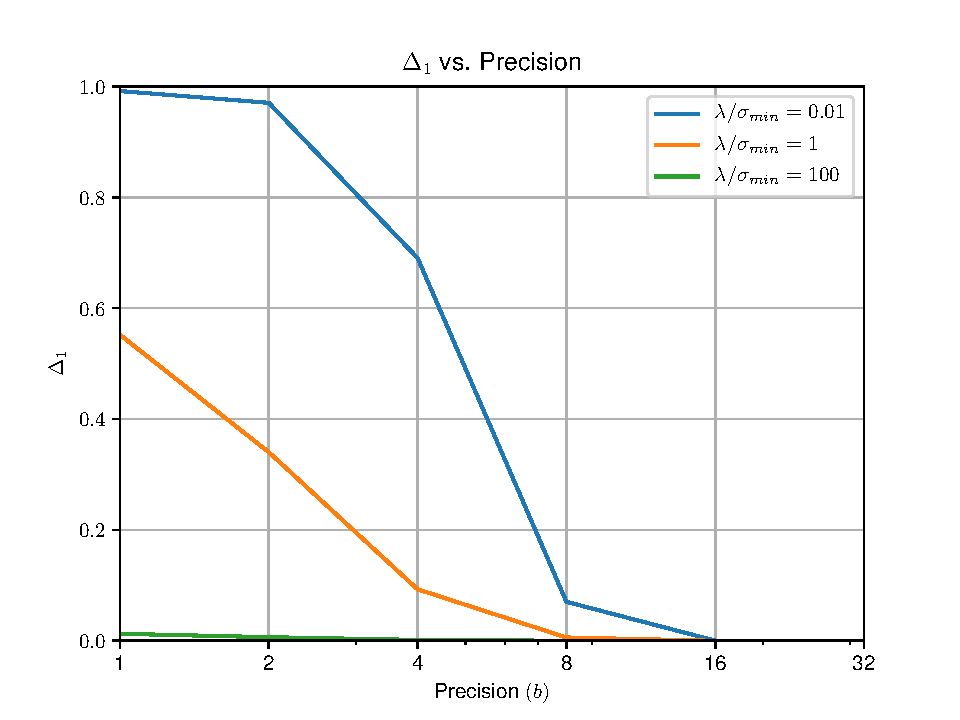
\includegraphics[width=0.45\linewidth]{figures/Delta1_vs_precision.pdf} &
		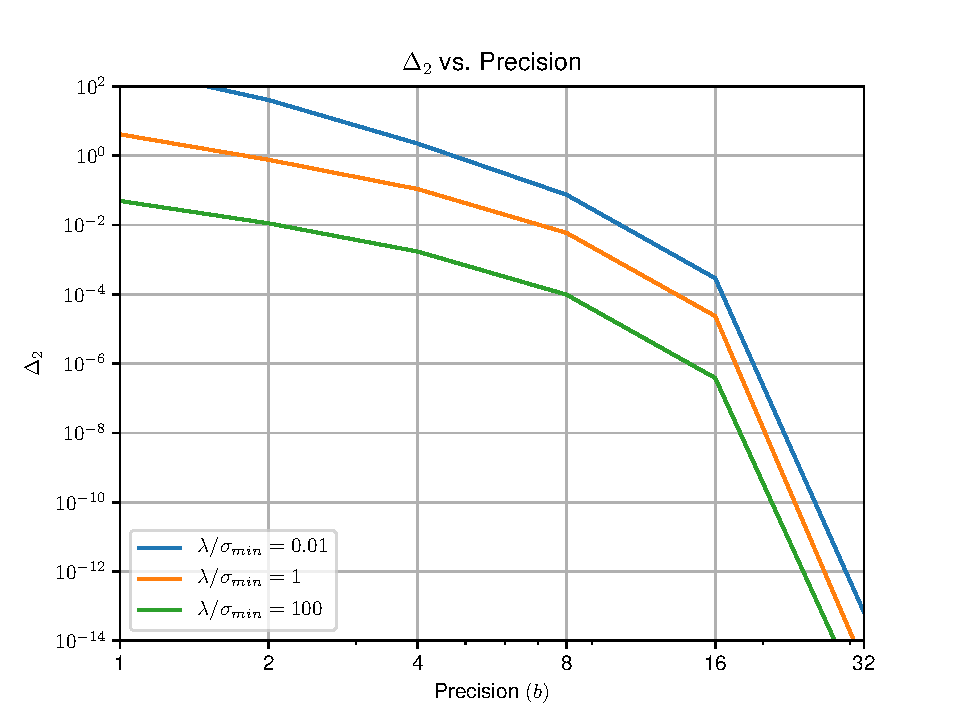
\includegraphics[width=0.45\linewidth]{figures/Delta2_vs_precision.pdf}
	\end{tabular}
	\label{fig:delta_vs_b}
	\caption{$\Delta1$ and $\Delta2$ as a function of quantization precision $b$ for uncompressed embedding $X$ and quantized embedding $\tilde{X}$. We can observe that $\Delta1$ and $\Delta2$ decreases as regularization strength $\lambda$ increases relative to $\sigma_{\min}$, the smallest eigenvalue of $XX^T$.}
\end{figure}



\begin{corollary}
	\label{cor:main2}
	If $\Delta_1 \geq \frac{\log(n/\rho)L}{3}\Big(1+\sqrt{1+\frac{18d}{\log(n/\rho)}}\Big) \approx 5n\cdot \frac{\delta_b}{\lambda}\sqrt{\frac{2\log(n/\rho)}{d}}$,
%	If $b \geq \log\left(\frac{5n}{\lambda \Delta_1} \sqrt{\frac{2\log(n/\rho)}{d}} \right)$,
	then $\Prob\big[(1 - \Delta_1) (K + \lambda I_n) \preceq \tK + \lambda I_n \big] \geq  1 - \rho$. 
	Similarly, if $\Delta_2 \geq \frac{\delta_b^2}{\lambda} +  \frac{\log(n/\rho)L}{3}\Big(1+\sqrt{1+\frac{18d}{\log(n/\rho)}}\Big) \approx \frac{\delta_b^2}{\lambda} + 5n\cdot \frac{\delta_b}{\lambda}\sqrt{\frac{2\log(n/\rho)}{d}}$,
%	Similarly, if $b \geq \log\left(\frac{1+5n}{\lambda \Delta_1} \sqrt{\frac{2\log(n/\rho)}{d}} \right)$
	then $\Prob\big[\tK + \lambda I_n \preceq (1 + \Delta_2) (K + \lambda I_n)\big] \geq  1 - \rho$. 
\end{corollary}


\todo{Should we also discuss the quantization noise small relative to regularizer setting?}

% the snippet for discussing large regularizer is OK here.
This corollary makes clear that if $\delta_b/\lambda$ is small, the $b$-bit compressed embedding matrix will be a close spectral approximation of the full-precision matrix, for small $\Delta_1$ and $\Delta_2$.
In the following theorem, we show that when the smallest singular value of $X^TX$ is large, using a large regularization parameter $\lambda$ will not significantly harm the generalization performance of $f_X$, relative to using a smaller $\lambda$.
%Combining this result with Proposition~\ref{prop:genbound} and Theorem~\ref{thm:main}, we can conclude that the generalization performance of a linear model trained on low-precision features with a large regularizer $\lambda$ will not be much worse than the performance of a model trained on the full-precision features with any $\lambda' \leq \lambda$.
%We now present the result:
%
%\begin{theorem}
%	\label{thm:large_lambda}
%	Let $X$ be an embedding matrix, and $\by$ be the corresponding vector of labels. Let $\sm$ be the smallest eigenvalue of $X^T X$, and let $\lambda', \lambda$ be two scalars such that $0 \leq \lambda' \leq \lambda \leq a\cdot \sm$, for some $a \in [0,1]$. Letting $\cR_{\lambda}(K)$ denote the expected loss when training with regularizer $\lambda$, Gram matrix $K = XX^T$, and label noise $\sigma^2$, we get that:
%	\begin{equation}
%	\frac{1}{\|y\|^2/n}\Big(R_{\lambda}(XX^T) - R_{\lambda'}(XX^T)\Big) \leq a^2
%	\label{eq1}
%	\end{equation}
%\end{theorem}
%Intuitively, this theorem shows that if there are no directions in the input space with very small variance, then using a large regularizer will not hurt performance significantly relative to using a smaller regularizer.
%This makes sense because the directions of small variance are the ones which are effectively ignored when strong regularization is used.
%For the purposes of this work, this theorem shows that if the embedding matrix has a large smallest eigenvalue, it should be possible to attain strong generalization performance with low-precision and a large regularizer.
%In practice, we observe that it is common for embedding matrices to have slowly decaying spectra, and thus have a large smallest eigenvalue;
%we present plots of the singular values for fastText and Glove embeddings in Figure~\ref{fig:real_spectra}.

\subsubsection{Empirical Validation}
\label{sec:theory_validation}
In this section, we empirically validate two important predictions made by the above theoretical results: (1) When $\delta_b/\lambda$ is small, $\Delta_1$ and $\Delta_2$ are small. (2) When $X^T X$ has a large smallest eigenvalue, generalization performance is not significantly harmed by using a large regularizer $\lambda$.
Lastly, we show that in general word embedding matrices have a relatively large smallest singular value;
combining this observation with the above theoretical results helps explain the strong performance of the uniformly quantized embeddings, even at very low precisions.

To validate the first prediction, we uniformly quantize a random matrix $X$ with various precisions $b$, and then measure the values of $\Delta_1$ and $\Delta_2$ for which the quantized Gram matrix is a $(\Delta_1,\Delta_2)$-spectral approximation of the full-precision Gram matrix.
More specifically, we randomly generate a matrix $X \in \RR^{1000 \times 30}$, where each entry is drawn uniformly from $[-\frac{1}{\sqrt{30}},\frac{1}{\sqrt{30}}]$.
We then uniformly quantize this matrix for precisions $b \in \{1,2,4,8,32\}$, denoting the quantized matrix by $\tX$.
Next, we compute the minimum values of $\Delta_1$ and $\Delta_2$ for which $\tX\tX^T + \lambda I$ is a $(\Delta_1,\Delta_2)$-spectral approximation of $XX^T + \lambda I$, for $\lambda \in \{2^{-32}, 2^{-24}, \ldots, 2^{12}, 2^{16}, 2^{20}\}$ \todo{Clean up this list of $\lambda$ values.}
In Figure~\ref{fig:micro_d1d2}, we plot the values of $\Delta_1$ and $\Delta_2$ as a function of $\delta_b/\lambda$, where $\delta_b \defeq 1/(2^b-1)$.
As we can see, the values of $\Delta_1$ and $\Delta_2$ are largely governed by the value of $\delta_b/\lambda$; when $\delta_b/\lambda$ is small, so are $\Delta_1$ and $\Delta_2$.

To validate the second prediction, we measure how the generalization error of a simple linear model grows as a function of the ratio between the regularization parameter $\lambda$ and the smallest eigenvalue of the covariance matrix $X^T X$.
Specifically, we consider the noiseless model $y = Xw^*$, where each entry of $X \in \RR^{1000 \times 2}$ is drawn from a zero-mean Gaussian with variance $\sigma^2$, and $w^*=[0,1]$.
Then, for various values of $\sigma$, and various values of $\lambda$, we learn the linear ridge regression model $w = (X^T X + \lambda I_d)^{-1}X^Ty$, and measure the mean-squared error $\|Xw-y\|_2^2$ as well as $\sigma_{\min}(X^T X)$.
Because we are in the noiseless setting, $\lambda'=0$ attains a mean-squared error of zero.
We are thus interested in understanding how quickly generalization performance degrades as $\lambda$ is increased to larger positive values.
In Figure~\ref{fig:micro_large_sigma_min} we plot the LHS of Equation~\eqref{eq1} as a function of the ratio $a \defeq \lambda/\sigma_{\min}$ for the various settings discussed above.
We see that when $a$ is small, the mean-squared error of the model trained with $\lambda$ performs similarly to using $\lambda'=0$, as predicted by the theory.

Lastly, in Figure~\ref{fig:real_spectra} we show that for real word embedding matrices the spectra decay quite slowly, such that the smallest eigenvalue is relatively large.
Combining this empirical observations with the theorems discussed above provides a principled explanation for why quantized word embeddings can attain strong empirical performance at such high compression rates.

\begin{figure*}
	\centering
	\begin{tabular}{c c}
		%		\begin{tabular}{@{\hskip -0.0in}c@{\hskip -0.0in}c@{\hskip -0.0in}c@{\hskip -0.0in}}
		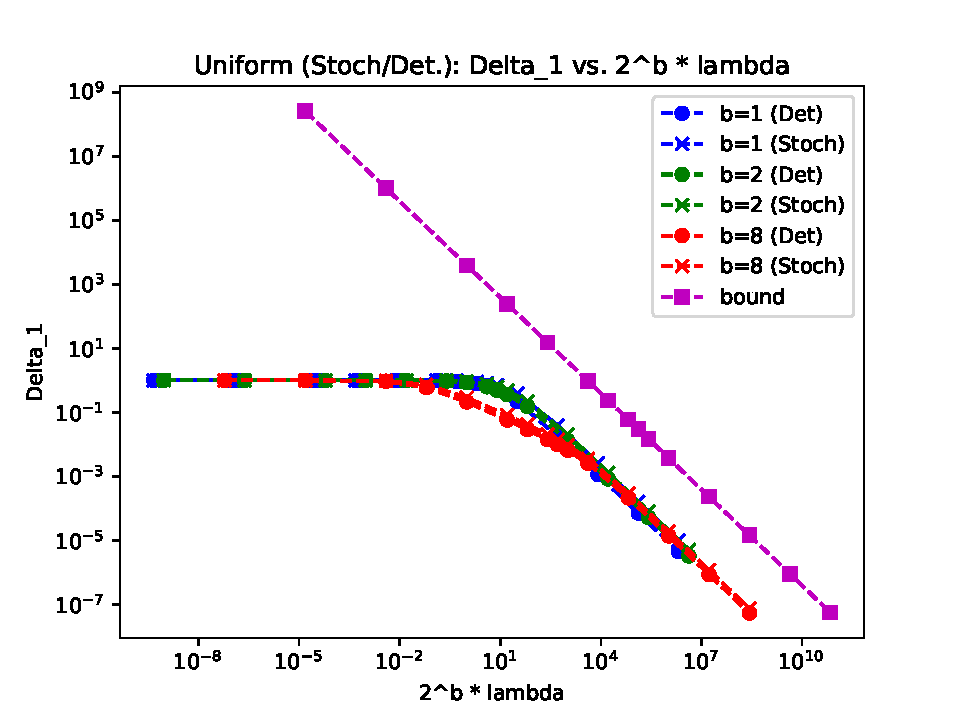
\includegraphics[width=0.4\linewidth]{figures/micro_uniform_nonadapt_delta1_vs_2_b_lambda.pdf} &	
		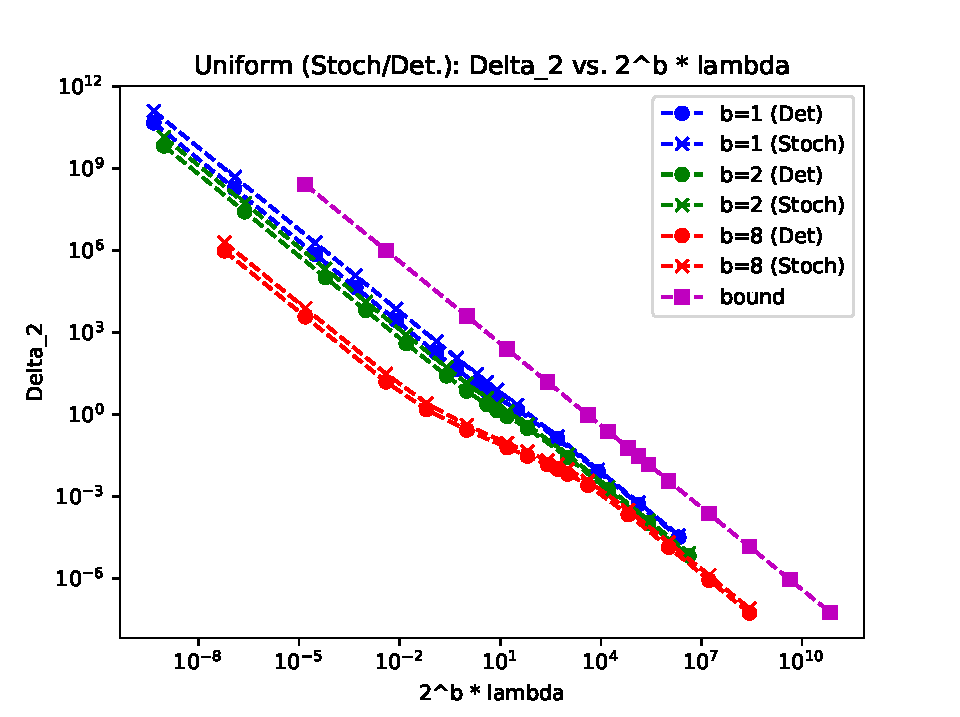
\includegraphics[width=0.4\linewidth]{figures/micro_uniform_nonadapt_delta2_vs_2_b_lambda.pdf}
	\end{tabular}
	\caption{We plot $\Delta_1$ (left) and $\Delta_2$ (right) as a function of $2^b\lambda$, on a randomly generated matrix $X\in\RR^{1000\times 30}$ ($X_{ij}\sim U([-\frac{1}{\sqrt{30}},\frac{1}{\sqrt{30}}])$), for various precisions $b$ and $\lambda$ values.  We show that $2^b \lambda$ largely determines the values of $\Delta_1$ and $\Delta_2$ after compression, as predicted by our theoretical results. We plot results for both deterministic quantization and stochastic quantization, and see that they perform quite similarly by these metrics (though deterministic does perform slightly better on $\Delta_2$). We additionally plot the bounds for $\Delta_1$ and $\Delta_2$ from Corollary~\ref{cor:main}, and see that while the bounds are not tight, their trajectory is matched by the real data.}
	\label{fig:micro_d1d2}
\end{figure*}

\begin{figure}
	\begin{center}
		\centerline{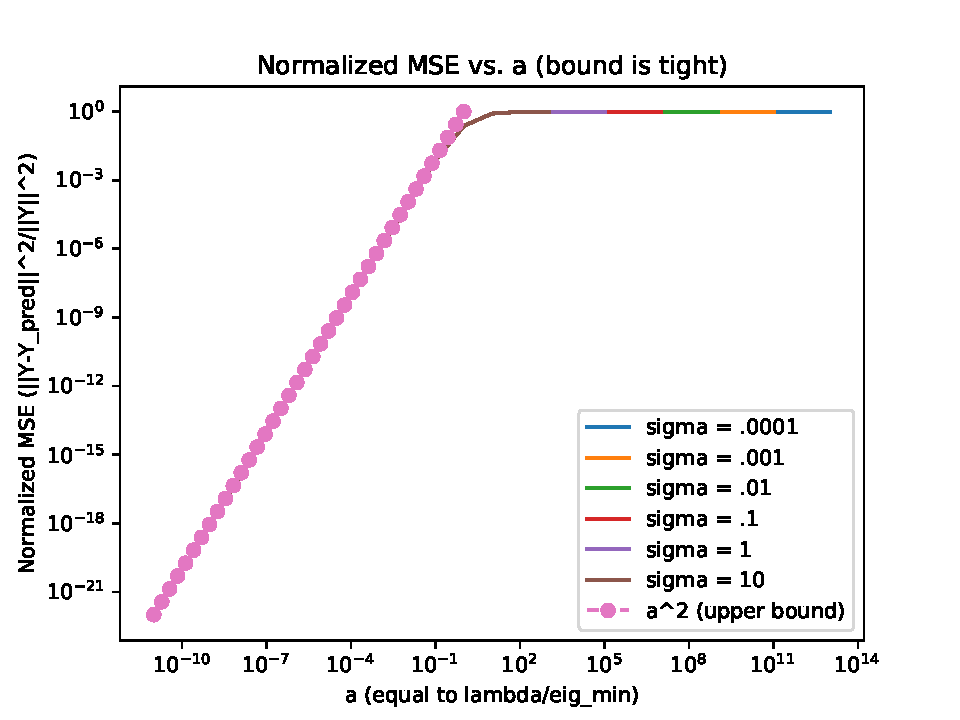
\includegraphics[width=0.8\columnwidth]{figures/micro_large_sigma_min.pdf}}
		\caption{We show that the ratio $a=\frac{\lambda}{\sigma_{\min}}$ between the regularization parameter $\lambda$ and the smallest eigenvalue $\sigma_{\min}$ of $X^T X$ is very predictive of the degradation in generalization performance $\|\by - y_{pred}\|^2/\|\by\|^2$, as predicted by Theorem~\ref{thm:large_lambda}.
		In particular, we generate an i.i.d. Gaussian matrix $X\in \RR^{1000\times 2}$ for various standard deviations $\sigma$, and consider the noiseless model $\by_i = [0,1]^T x_i$.
		We then solve for the optimal ridge regression model for various values of $\lambda$, and plot $a$ vs.\ the normalized degradation in generalization performance of this model. \todo{TODO: Perhaps plot a more realistic example?  And use $\|\by - y_{pred}\|^2/(\|\by\|^2/n)$ as y-axis.}
		}
		\label{fig:micro_large_sigma_min}
	\end{center}
\end{figure}

\begin{figure*}
	\centering
	\begin{tabular}{c c}
		%		\begin{tabular}{@{\hskip -0.0in}c@{\hskip -0.0in}c@{\hskip -0.0in}c@{\hskip -0.0in}}
		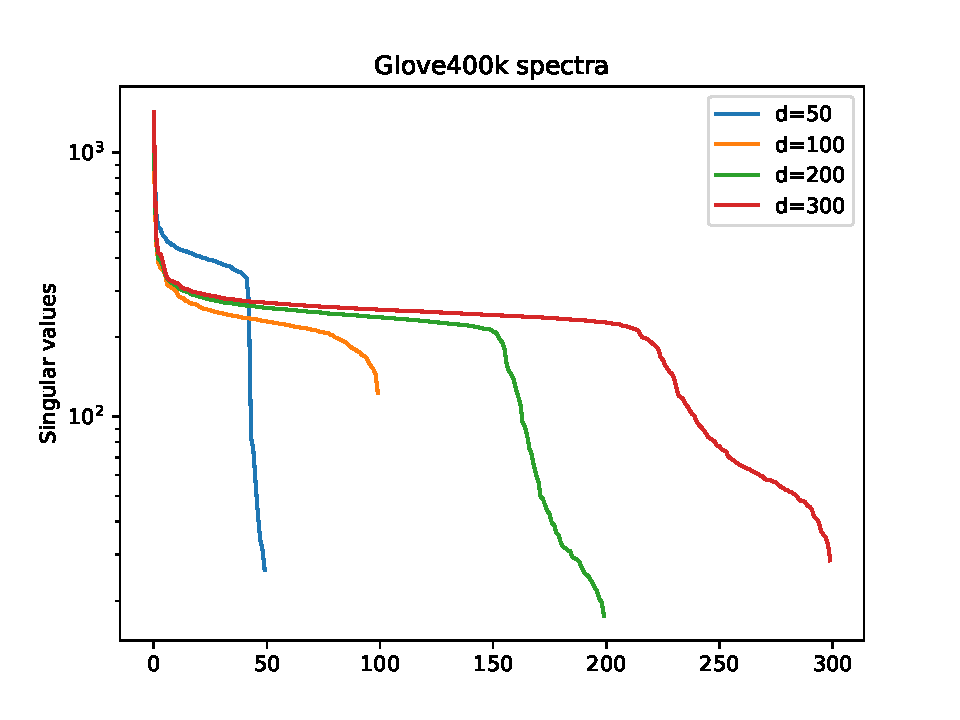
\includegraphics[width=0.4\linewidth]{figures/glove400k_spectra.pdf} &	
		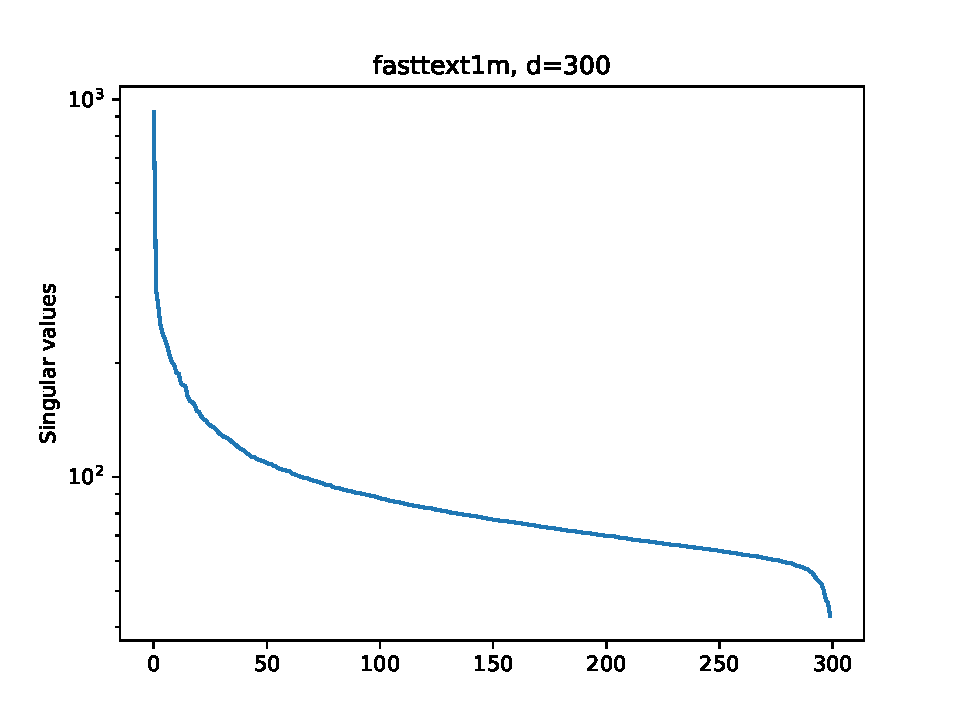
\includegraphics[width=0.4\linewidth]{figures/fasttext1m_spectra.pdf}
	\end{tabular}
	\caption{We plot the real spectra of the pre-trained GloVe ($d \in \{50,100,200,300\}$) and fastText ($d=300$) embedding matrices.
	The smallest singular values are generally only 1 or 2 orders of magnitude smaller than the largest.  
	\todo{Add spectra for GloVe embeddings we trained from scratch ($d\in\{25,50,100,200,400\}$).}}
	\label{fig:real_spectra}
\end{figure*}

\subsubsection{Effect of Clipping on $(\Delta_1,\Delta_2)$}
\label{sec:theory_clipping}
One way to understand why it is important for us to search for the optimal clipping value in Algorithm~\ref{alg:smallfry} is by understanding the way clipping and quantization together impact $\Delta_1$ and $\Delta_2$.
This perspective reveals that there is a fundamental trade-off between $\Delta_1$ and $\Delta_2$ when choosing the clipping value:
if the clip value is too large, then $\Delta_2$ becomes very large, while if the clip value is too small, then $\Delta_1$ becomes very large.
We demonstrate this in Figure~\ref{fig:deltas_vs_clip_quant}.
\todo{Polish and expand the discussion here, and discuss how using Frobenius error to pick optimal clipping value leads to a nice point on the trade-off curve between $\Delta_1$ and $\Delta_2$.}
\begin{figure}
	\begin{center}
		\centerline{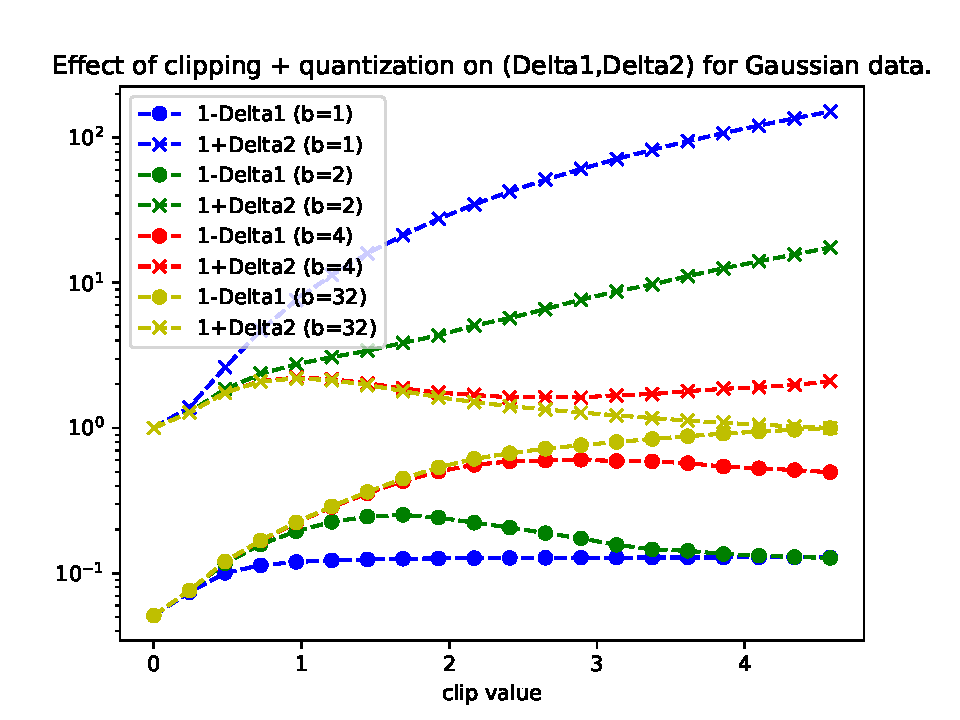
\includegraphics[width=0.8\columnwidth]{figures/deltas_vs_clip_and_quant.pdf}}
		\caption{On random Gaussian data $X \in \RR^{1000\times 30}$, we demonstrate the joint effect of clipping and quantizing on $\Delta_1$ and $\Delta_2$, where we take $\lambda = \sigma_{\min}(X^T X)/10$.
		A large clipping value gives large $\Delta_2$, whereas a small clipping values gives large $\Delta_1$.
		This reveals the importance of choosing a clipping value which balances these two considerations.
		}
		\label{fig:deltas_vs_clip_quant}
	\end{center}
\end{figure}


%In this section, we analyze in the context of linear ridge regression how the dimension and precision of uniformly quantized word embeddings jointly impact generalization performance.
%Though linear regression is evidently a very simplified setting, we believe the analysis in this setting is an important first step toward understanding the way compression affects generalization performance on downstream tasks.
%We present two main results:
%First, we show there is a bias-variance trade-off when choosing the embedding dimension, and that there can thus be an optimal dimension.
%We then show that quantized embeddings can attain comparable generalization performance to full-precision embeddings at high compression rates when the spectrum of the embedding matrix decays slowly (which we empirically observe to be true).
%Combined, these two results imply that one can attain large improvements in generalization performance in the memory constrained setting by using low-precision embeddings whose dimension approaches but does not exceed the optimal dimension.
%
%%In this section, we present generalization bounds for linear regression models trained on top of uniformly quantized word embeddings.
%%Though linear regression is evidently a very simplified setting, we believe the analysis in this setting is an important first step toward understanding the way compression affects generalization performance on downstream tasks.
%%We present two main results:
%%First, we show that when the standard deviation of the quantization noise is small relative to the regularization parameter $\lambda$ used to train the linear model, we attain good generalization bounds for the quantized embeddings relative to the full-precision embeddings.
%%Second, we show that if the singular values of the embedding matrix decay slowly, then training the regression model with a large regularization parameter $\lambda$ cannot perform much worse than training with a smaller one.
%%Combining these two results with our empirical observation that word embedding spectra decay relatively slowly helps explain why quantized word embeddings perform so well at high compression rates.
%
%This section is organized as follows:
%In Section~\ref{sec:theory_dim} we review fixed design linear ridge regression and discuss the trade-off involved in choosing the embedding dimension.
%In Section~\ref{sec:theory_quantization} we present our analysis on the impact of quantization on generalization performance.
%
%\subsection{Generalization and Dimensionality}
%\label{sec:theory_dim}
%
%\subsubsection{Background: Generalization Bounds for Fixed Design Linear Regression}
%In fixed design linear regression, one is given a dataset $\{(x_i,y_i)\}_{i=1}^n$, for $x_i \in \RR^d$ and $y_i = \by_i + \eps_i \in \RR$, where the $\eps_i$ are independent random perturbations of the ``true labels'' $\by_i$ satisfying $\expect{}{\eps_i} = 0$ and $\var{}{\eps_i} = \sigma^2 < \infty$.
%The goal is to design a training algorithm which takes as input the noisy dataset $\{(x_i,y_i)\}_{i=1}^n$ and outputs a model $f(x) = w^T x$ for which $\expect{}{\frac{1}{n}\sum_i (f(x_i) -\by_i)^2} \eqdef \cR(f)$ is small.
%Linear ridge regression selects $w^* = \argmin_w \sum_i (w^T x_i - y_i)^2 + \lambda\|w\|_2^2$.
%Letting $X \in \RR^{n\times d}$ be the matrix whose rows are $x_i$, $y \defeq (y_1,...,y_n) \in \RR^d$, and $I_d$ be the $d$-dimensional identity matrix, the minimizer of this optimization problem is $w^* = ( X^T X + \lambda I_d)^{-1}X^Ty$.
%It is easy to show \citep{alaoui15} that the expected generalization error for the model $f_X(x) \defeq w^{*T}x$ is
%\begin{eqnarray*}
%\cR(f_X) &=& \frac{\lambda^2}{n} \by^T(XX^T + \lambda I_n)^{-2}\by \; +\\ && \frac{\sigma^2}{n}\tr\Big((XX^T)^2(XX^T + \lambda I_n)^{-2}\Big)\\
%&=& \text{``bias''} + \text{``variance''}.
%\end{eqnarray*}
%
%\subsubsection{Choice of Embedding Dimension}
%We now discuss how the choice of dimension affects the bias and variance terms in the above expression for generalization performance.
%To perform this analysis, we will take the common approach of viewing word embedding as a matrix factorization problem, for example of a positive pointwise mutual information (PPMI) matrix \citep{levy14}.
%In particular, we will assume that the $d$-dimensional embedding $X_d$ is computed via a low-rank decomposition of an $n$-by-$n$ matrix $K = U \Sigma U^T$, where $X_d = U_{1:d} \Sigma_{1:d}^{1/2}$ is the product of the first $d$ eigenvectors and eigenvalues.
%Denoting the $i^{th}$ largest eigenvalue by $\sigma_i$ and the corresponding eigenvector by $U_i$, we can rewrite the bias and variance terms as follows:
%\begin{eqnarray*}
%\hspace{-0.2in}&&\text{``bias''} = \frac{1}{n}\sum_{i=1}^d \bigg(\frac{\lambda}{\sigma_i + \lambda}\bigg)^2 \Big(U_i^T \by \Big)^2 + \frac{1}{n}\sum_{i=d+1}^n \Big(U_i^T \by \Big)^2\\
%\hspace{-0.2in}&&\text{``variance''} = \frac{\sigma^2}{n}\sum_{i=1}^d \bigg(\frac{\sigma_i}{\sigma_i + \lambda}\bigg)^2.
%\end{eqnarray*}
%As we can see, incrementing the dimension from $d-1$ to $d$ will decrease the bias term by $\frac{1}{n}(U_d^T \by)^2\big(1-\big(\frac{\lambda}{\sigma_d + \lambda}\big)^2\big)$,
%while increasing the variance term by $\frac{\sigma^2}{n}\big(\frac{\sigma_d}{\sigma_d + \lambda}\big)^2$.
%This suggests that there could be an optimal dimension, beyond which adding more features would increase the variance more than it would decrease the bias.
%\todo{This occurs if all the entries beyond $i=d^*$ in the sequence $\frac{\sigma_i}{\sigma_i + \lambda}$ are larger than those in the sequence $\frac{2 (U_i^T\by)^2}{\sigma^2 + (U_i^T\by)^2}$ (and if the opposite is true for all entries $d^*$ and below). For more details, see Appendix.}
%
%\subsubsection{Empirical Validation}
%\todo{Add empirical validation of the impact of dimension on performance.}
%
%\subsection{Generalization and Quantization}
%\label{sec:theory_quantization}
%
%\subsubsection{Background: Performance of Approximate Features}
%Here, we present generalization bounds for models trained on top of an approximation $\tX$ to the true data matrix $X$, as this will allow us to analyze the impact of quantization on generalization performance.
%To derive these bounds, we intuitively require two things: a notion of distance between $X$ and $\tX$, and an upper bound for $\cR(f_{\tX})$ in terms of $\cR(f_X)$ and the distance between $X$ and $\tX$.
%For both of these components, we leverage the recent work of \citep{lprff18}.
%In that work, they define the following notion of distance between two matrices:
%
%\begin{definition}{\citep{lprff18}}
%	\label{def:specdist}
%	For $\Delta_1, \Delta_2 \geq 0$, a symmetric matrix $A$ is a \emph{$(\Delta_1, \Delta_2)$-spectral approximation} of another symmetric matrix $B$ if $(1-\Delta_1)B \preceq A \preceq (1+\Delta_2)B$. 
%\end{definition}
%
%By applying this definition to $\tX\tX^T + \lambda I_n$ and $XX^T + \lambda I_n$, the authors prove the following generalization bound:
%\begin{proposition}{(Adapted from \citep{lprff18})}
%	Let $K \defeq XX^T$ and $\tK \defeq \tX\tX^T$, and suppose $\tK + \lambda I_n$ is $(\Delta_1, \Delta_2)$-spectral approximation of $K+\lambda I_n$, for $\Delta_1 \in [0,1)$, $\Delta_2 \geq 0$.
%	Let $d$ denote the rank of $\tX$, and let $f_{X}$ and $f_{\tX}$ be the ridge regression estimators learned using these matrices, with regularizing constant $\lambda \geq 0$ and label noise variance $\sigma^2 < \infty$. Then
%	\begin{equation}
%	\cR(f_{\tX}) \leq \frac{1}{1-\Delta_1} \hcR(f_X) +  \frac{\Delta_2}{1+\Delta_2}\frac{d}{n}\sigma^2,
%	\label{eq:risk_bound}
%	\end{equation}
%	where 
%	\begin{eqnarray*}
%	\hcR(f_X) &\defeq& \frac{\lambda}{n} \by^T(K+\lambda I)^{-1}\by + \frac{\sigma^2}{n}\tr\Big(K(K+\lambda I)^{-1}\Big) \\
%	&\geq& \cR(f_X).
%%	\label{eq:avron_rhat}
%	\end{eqnarray*}
%	\label{prop:genbound}
%\end{proposition}
%% HERE IS THE OTHER VERSION OF THE GENERALIZATION BOUND
%%\subsection{New bound}
%%\begin{eqnarray*}
%%	R(\tf) &=& \frac{\lambda^2}{n}y^T(\tK + \lambda I)^{-2}y + \frac{\sigma^2}{n}\tr\bigg(\tK^2(\tK + \lambda I)^{-2}\bigg)\\
%%	&=& \frac{\lambda^2}{n}y^T(\tK + \lambda I)^{-2}y + \frac{\sigma^2}{n}\sum_{i=1}^d \bigg(\frac{\sigma_i}{\sigma_i + \lambda}\bigg)^2 \\
%%	&\leq& \frac{\lambda^2}{n}y^T(\tK + \lambda I)^{-2}y + \frac{\sigma^2d}{n} \\
%%	&\leq& \frac{\lambda}{n}y^T(\tK + \lambda I)^{-1}y + \frac{\sigma^2d}{n} \\
%%	&\leq& \frac{1}{1-\Delta_1}\cdot \frac{\lambda}{n}y^T(K + \lambda I)^{-1}y + \frac{\sigma^2d}{n} \\
%%	&=& \frac{1}{1-\Delta_1}R'(f) + \frac{\sigma^2d}{n},\quad\text{where} \\
%%	R'(f) &\defeq& \frac{\lambda}{n}y^T(K + \lambda I)^{-1}y \\
%%	&\geq& \frac{\lambda^2}{n}y^T(K + \lambda I)^{-2}y \;\;\;\text{(emp. loss of f.p. embeddings.)}
%%\end{eqnarray*}
%
%
%%\todo{Discuss how what we will show differs from what is shown in kernel paper.}
%
%\subsubsection{Theoretical Results: Effect of Quantization}
%\label{sec:theory_results}
%We now show that our compression algorithm with high probability produces an embedding matrix which is a close spectral approximation of the full-precision matrix, in terms of $(\Delta_1,\Delta_2)$.
%Combining this with the Proposition~\ref{prop:genbound} yields a generalization bound for the compressed embeddings.
%A consequence of our bound is that when the regularization parameter is large, lower precision can be used for the embeddings without affecting $\Delta_1$ and $\Delta_2$.
%We show that in the case of word embeddings with slowly-decaying singular values, a large regularization parameter $\lambda$ (and thus, a low-precision $b$) can be used without significantly affecting generalization performance.
%Our empirical observation that embedding matrices have slowly decaying singular values thus helps explain why our compression algorithm is able to attain strong generalization performance at very low levels of precision.
%
%We now present our main theoretical result, deferring all proofs to the Appendix:
%\begin{theorem}
%	\label{thm:main}
%	Let $X \in \RR^{n\times d}$ be an embedding matrix with corresponding Gram matrix $K \defeq XX^T$, where we assume all entries $X_{ij} \in [-\frac{1}{\sqrt{d}},\frac{1}{\sqrt{d}}]$; let $\tX\defeq X+C$ denote a $b$-bit quantization of $X$, with $\tK \defeq \tX\tX^T$ the kernel matrix of the quantized data matrix. Here, $C$ denotes the quantization noise, with $\expect{}{C_{ij}} = 0$ and $\var{}{C_{ij}} \leq \delta_b^2/d \;\;\forall i,j$, where $\delta_b^2 \defeq (2^b-1)^{-2}$, and $b$ is the number of bits used per feature.
%	Then for any $\Delta_1 \geq 0, \Delta_2 \geq \delta^2_b/\lambda$,
%	\begin{eqnarray*}
%	&&\hspace{-0.37in}\Prob\Big[(1- \Delta_1) (K + \lambda I_n) \preceq \tK + \lambda I_n \preceq (1 + \Delta_2) (K + \lambda I_n)
%	\Big] 
%	\\ &\geq& 1 - 
%	n \exp \bigg(\frac{-\Delta_1^2}{2dL^2 + (2L/3)\Delta_1}\bigg) \\
%	&&- n \exp \bigg(\frac{-(\Delta_2-\delta_b^2/\lambda)^2}{2dL^2 + (2L/3)(\Delta_2-\delta_b^2/\lambda)}\bigg),
%	\end{eqnarray*}
%	for $L \defeq 5 \cdot \frac{2^b \cdot \delta_b^2}{\lambda}\cdot \frac{n}{d}$.
%\end{theorem}
%Note that in this theorem, we assume the embedding matrix is bounded, whereas in the actual implementation of our compression algorithm (Alg.~\ref{alg:smallfry}) we enforce this constraint artificially by searching for the optimal threshold at which to clip the matrix entries.
%\todo{Say more about boundedness assumption.}
%To better understand the implications of the above theorem, we present the following corollary:
%\begin{corollary}
%	\label{cor:main}
%%	If $\Delta_1 \geq \frac{\log(n/\rho)L}{3}\Big(1+\sqrt{1+\frac{18d}{\log(n/\rho)}}\Big) \approx 5n\cdot \frac{\delta_b}{\lambda}\sqrt{\frac{2\log(n/\rho)}{d}}$,
%	If $b \geq \log\left(\frac{5n}{\lambda \Delta_1} \sqrt{\frac{2\log(n/\rho)}{d}} \right)$,
%	then $\Prob\big[(1 - \Delta_1) (K + \lambda I_n) \preceq \tK + \lambda I_n \big] \geq  1 - \rho$. 
%%	Similarly, if $\Delta_2 \geq \frac{\delta_b^2}{\lambda} +  \frac{\log(n/\rho)L}{3}\Big(1+\sqrt{1+\frac{18d}{\log(n/\rho)}}\Big) \approx \frac{\delta_b^2}{\lambda} + 5n\cdot \frac{\delta_b}{\lambda}\sqrt{\frac{2\log(n/\rho)}{d}}$,
%	Similarly, if $b \geq \log\left(\frac{1+5n}{\lambda \Delta_1} \sqrt{\frac{2\log(n/\rho)}{d}} \right)$
%	then $\Prob\big[\tK + \lambda I_n \preceq (1 + \Delta_2) (K + \lambda I_n)\big] \geq  1 - \rho$. 
%\end{corollary}
%
%
%This corollary makes clear that if $\delta_b/\lambda$ is small, the $b$-bit compressed embedding matrix will be a close spectral approximation of the full-precision matrix, for small $\Delta_1$ and $\Delta_2$.
%In the following theorem, we show that when the smallest singular value of $X^TX$ is large, using a large regularization parameter $\lambda$ will not significantly harm the generalization performance of $f_X$, relative to using a smaller $\lambda$.
%Combining this result with Proposition~\ref{prop:genbound} and Theorem~\ref{thm:main}, we can conclude that the generalization performance of a linear model trained on low-precision features with a large regularizer $\lambda$ will not be much worse than the performance of a model trained on the full-precision features with any $\lambda' \leq \lambda$.
%We now present the result:
%
%\begin{theorem}
%	\label{thm:large_lambda}
%	Let $X$ be an embedding matrix, and $\by$ be the corresponding vector of labels. Let $\sm$ be the smallest eigenvalue of $X^T X$, and let $\lambda', \lambda$ be two scalars such that $0 \leq \lambda' \leq \lambda \leq a\cdot \sm$, for some $a \in [0,1]$. Letting $\cR_{\lambda}(K)$ denote the expected loss when training with regularizer $\lambda$, Gram matrix $K = XX^T$, and label noise $\sigma^2$, we get that:
%	\begin{equation}
%	\frac{1}{\|y\|^2/n}\Big(R_{\lambda}(XX^T) - R_{\lambda'}(XX^T)\Big) \leq a^2
%	\label{eq1}
%	\end{equation}
%\end{theorem}
%Intuitively, this theorem shows that if there are no directions in the input space with very small variance, then using a large regularizer will not hurt performance significantly relative to using a smaller regularizer.
%This makes sense because the directions of small variance are the ones which are effectively ignored when strong regularization is used.
%For the purposes of this work, this theorem shows that if the embedding matrix has a large smallest eigenvalue, it should be possible to attain strong generalization performance with low-precision and a large regularizer.
%In practice, we observe that it is common for embedding matrices to have slowly decaying spectra, and thus have a large smallest eigenvalue;
%we present plots of the singular values for fastText and Glove embeddings in Figure~\ref{fig:real_spectra}.
%
%\subsubsection{Empirical Validation}
%\label{sec:theory_validation}
%In this section, we empirically validate two important predictions made by the above theoretical results: (1) When $\delta_b/\lambda$ is small, $\Delta_1$ and $\Delta_2$ are small. (2) When $X^T X$ has a large smallest eigenvalue, generalization performance is not significantly harmed by using a large regularizer $\lambda$.
%Lastly, we show that in general word embedding matrices have a relatively large smallest singular value;
%combining this observation with the above theoretical results helps explain the strong performance of the uniformly quantized embeddings, even at very low precisions.
%
%To validate the first prediction, we uniformly quantize a random matrix $X$ with various precisions $b$, and then measure the values of $\Delta_1$ and $\Delta_2$ for which the quantized Gram matrix is a $(\Delta_1,\Delta_2)$-spectral approximation of the full-precision Gram matrix.
%More specifically, we randomly generate a matrix $X \in \RR^{1000 \times 30}$, where each entry is drawn uniformly from $[-\frac{1}{\sqrt{30}},\frac{1}{\sqrt{30}}]$.
%We then uniformly quantize this matrix for precisions $b \in \{1,2,4,8,32\}$, denoting the quantized matrix by $\tX$.
%Next, we compute the minimum values of $\Delta_1$ and $\Delta_2$ for which $\tX\tX^T + \lambda I$ is a $(\Delta_1,\Delta_2)$-spectral approximation of $XX^T + \lambda I$, for $\lambda \in \{2^{-32}, 2^{-24}, \ldots, 2^{12}, 2^{16}, 2^{20}\}$ \todo{Clean up this list of $\lambda$ values.}
%In Figure~\ref{fig:micro_d1d2}, we plot the values of $\Delta_1$ and $\Delta_2$ as a function of $\delta_b/\lambda$, where $\delta_b \defeq 1/(2^b-1)$.
%As we can see, the values of $\Delta_1$ and $\Delta_2$ are largely governed by the value of $\delta_b/\lambda$; when $\delta_b/\lambda$ is small, so are $\Delta_1$ and $\Delta_2$.
%
%To validate the second prediction, we measure how the generalization error of a simple linear model grows as a function of the ratio between the regularization parameter $\lambda$ and the smallest eigenvalue of the covariance matrix $X^T X$.
%Specifically, we consider the noiseless model $y = Xw^*$, where each entry of $X \in \RR^{1000 \times 2}$ is drawn from a zero-mean Gaussian with variance $\sigma^2$, and $w^*=[0,1]$.
%Then, for various values of $\sigma$, and various values of $\lambda$, we learn the linear ridge regression model $w = (X^T X + \lambda I_d)^{-1}X^Ty$, and measure the mean-squared error $\|Xw-y\|_2^2$ as well as $\sigma_{\min}(X^T X)$.
%Because we are in the noiseless setting, $\lambda'=0$ attains a mean-squared error of zero.
%We are thus interested in understanding how quickly generalization performance degrades as $\lambda$ is increased to larger positive values.
%In Figure~\ref{fig:micro_large_sigma_min} we plot the LHS of Equation~\eqref{eq1} as a function of the ratio $a \defeq \lambda/\sigma_{\min}$ for the various settings discussed above.
%We see that when $a$ is small, the mean-squared error of the model trained with $\lambda$ performs similarly to using $\lambda'=0$, as predicted by the theory.
%
%Lastly, in Figure~\ref{fig:real_spectra} we show that for real word embedding matrices the spectra decay quite slowly, such that the smallest eigenvalue is relatively large.
%Combining this empirical observations with the theorems discussed above provides a principled explanation for why quantized word embeddings can attain strong empirical performance at such high compression rates.
%
%\begin{figure*}
%	\centering
%	\begin{tabular}{c c}
%		%		\begin{tabular}{@{\hskip -0.0in}c@{\hskip -0.0in}c@{\hskip -0.0in}c@{\hskip -0.0in}}
%		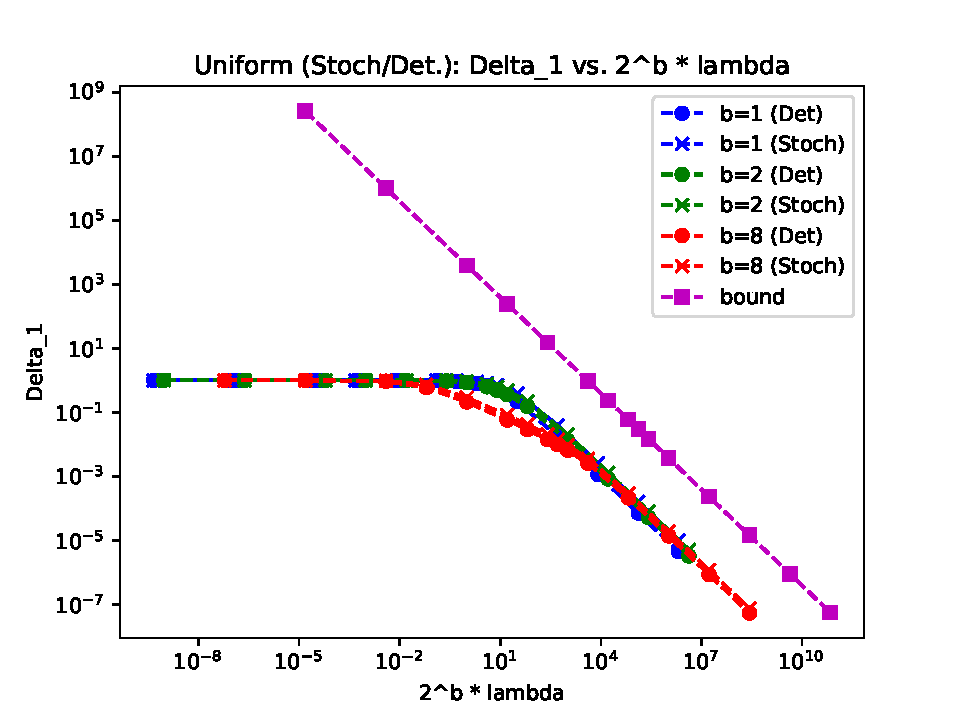
\includegraphics[width=0.4\linewidth]{figures/micro_uniform_nonadapt_delta1_vs_2_b_lambda.pdf} &	
%		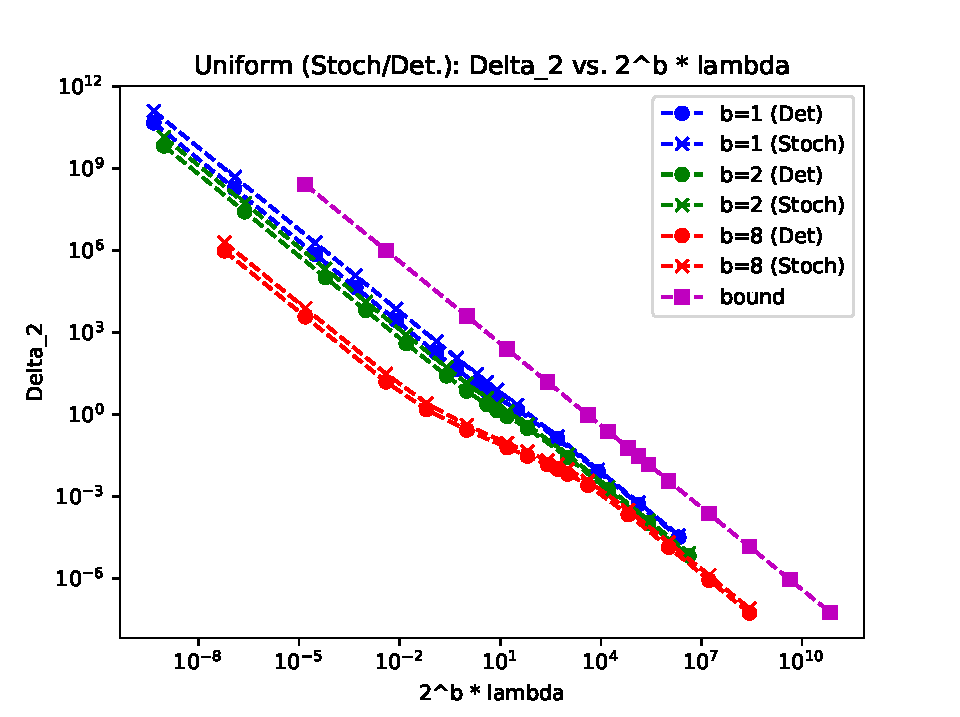
\includegraphics[width=0.4\linewidth]{figures/micro_uniform_nonadapt_delta2_vs_2_b_lambda.pdf}
%	\end{tabular}
%	\caption{We plot $\Delta_1$ (left) and $\Delta_2$ (right) as a function of $2^b\lambda$, on a randomly generated matrix $X\in\RR^{1000\times 30}$ ($X_{ij}\sim U([-\frac{1}{\sqrt{30}},\frac{1}{\sqrt{30}}])$), for various precisions $b$ and $\lambda$ values.  We show that $2^b \lambda$ largely determines the values of $\Delta_1$ and $\Delta_2$ after compression, as predicted by our theoretical results. We plot results for both deterministic quantization and stochastic quantization, and see that they perform quite similarly by these metrics (though deterministic does perform slightly better on $\Delta_2$). We additionally plot the bounds for $\Delta_1$ and $\Delta_2$ from Corollary~\ref{cor:main}, and see that while the bounds are not tight, their trajectory is matched by the real data.}
%	\label{fig:micro_d1d2}
%\end{figure*}
%
%\begin{figure}
%	\begin{center}
%		\centerline{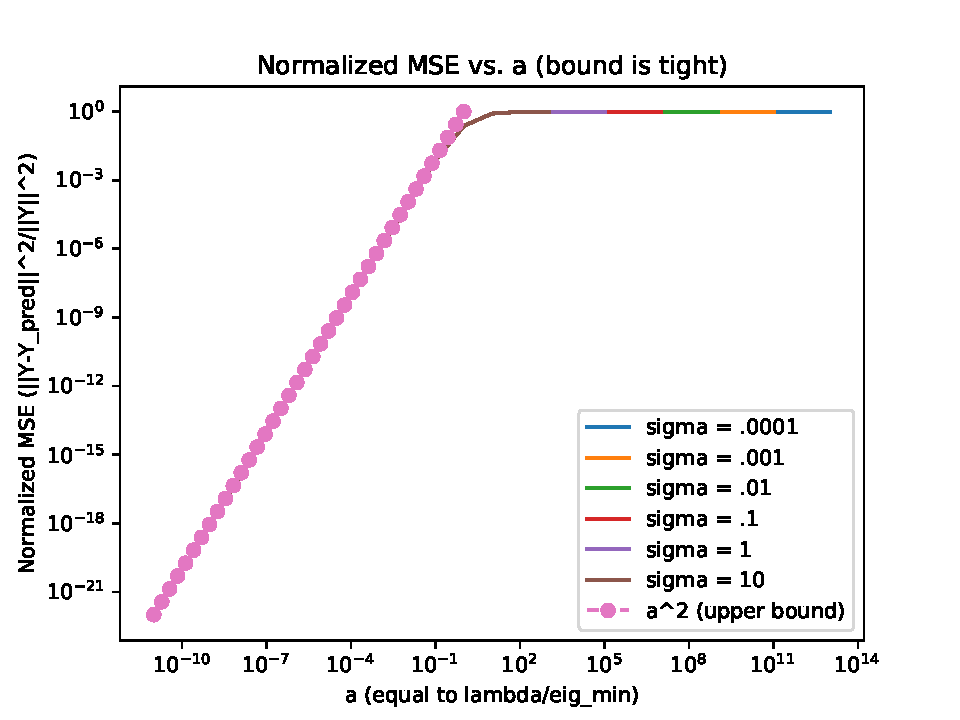
\includegraphics[width=0.8\columnwidth]{figures/micro_large_sigma_min.pdf}}
%		\caption{We show that the ratio $a=\frac{\lambda}{\sigma_{\min}}$ between the regularization parameter $\lambda$ and the smallest eigenvalue $\sigma_{\min}$ of $X^T X$ is very predictive of the degradation in generalization performance $\|\by - y_{pred}\|^2/\|\by\|^2$, as predicted by Theorem~\ref{thm:large_lambda}.
%		In particular, we generate an i.i.d. Gaussian matrix $X\in \RR^{1000\times 2}$ for various standard deviations $\sigma$, and consider the noiseless model $\by_i = [0,1]^T x_i$.
%		We then solve for the optimal ridge regression model for various values of $\lambda$, and plot $a$ vs.\ the normalized degradation in generalization performance of this model. \todo{TODO: Perhaps plot a more realistic example?  And use $\|\by - y_{pred}\|^2/(\|\by\|^2/n)$ as y-axis.}
%		}
%		\label{fig:micro_large_sigma_min}
%	\end{center}
%\end{figure}
%
%\begin{figure*}
%	\centering
%	\begin{tabular}{c c}
%		%		\begin{tabular}{@{\hskip -0.0in}c@{\hskip -0.0in}c@{\hskip -0.0in}c@{\hskip -0.0in}}
%		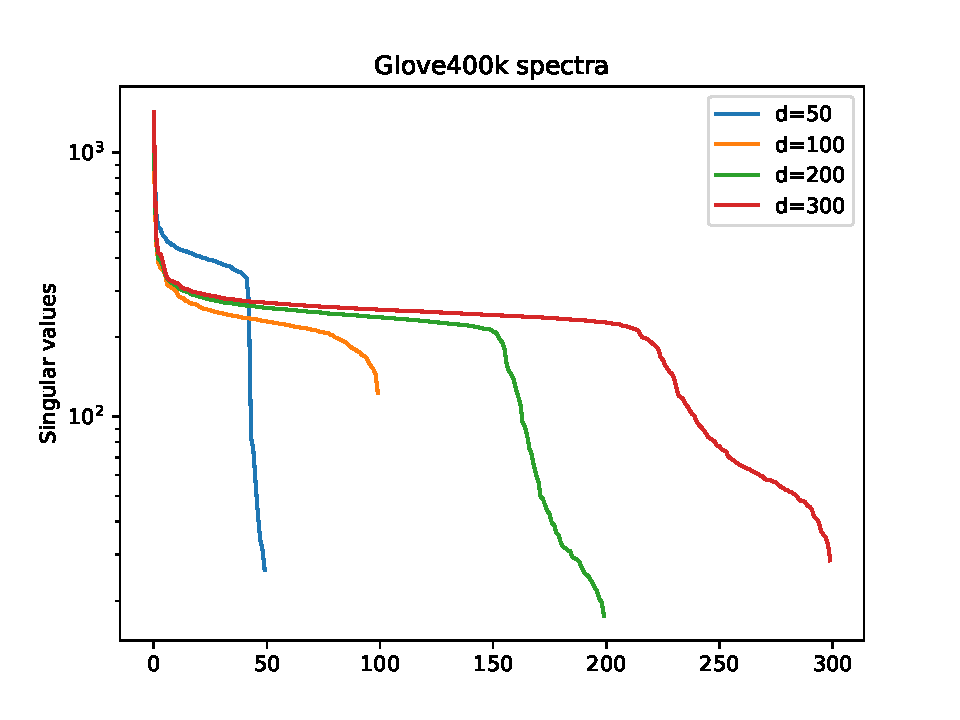
\includegraphics[width=0.4\linewidth]{figures/glove400k_spectra.pdf} &	
%		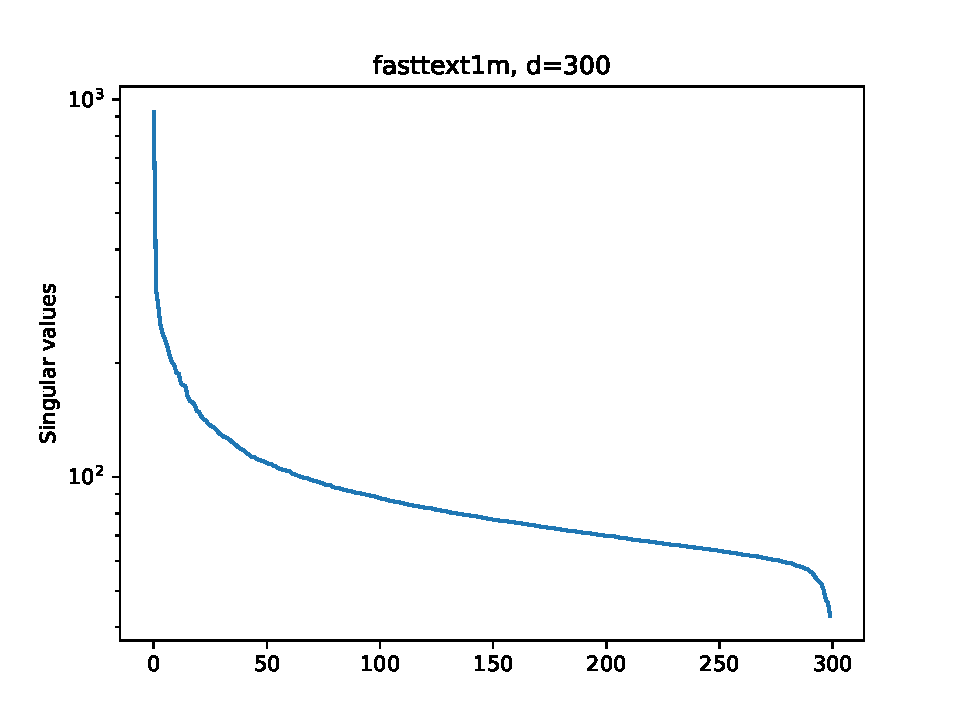
\includegraphics[width=0.4\linewidth]{figures/fasttext1m_spectra.pdf}
%	\end{tabular}
%	\caption{We plot the real spectra of the pre-trained GloVe ($d \in \{50,100,200,300\}$) and fastText ($d=300$) embedding matrices.
%	The smallest singular values are generally only 1 or 2 orders of magnitude smaller than the largest.  
%	\todo{Add spectra for GloVe embeddings we trained from scratch ($d\in\{25,50,100,200,400\}$).}}
%	\label{fig:real_spectra}
%\end{figure*}
%
%\subsubsection{Effect of Clipping on $(\Delta_1,\Delta_2)$}
%\label{sec:theory_clipping}
%One way to understand why it is important for us to search for the optimal clipping value in Algorithm~\ref{alg:smallfry} is by understanding the way clipping and quantization together impact $\Delta_1$ and $\Delta_2$.
%This perspective reveals that there is a fundamental trade-off between $\Delta_1$ and $\Delta_2$ when choosing the clipping value:
%if the clip value is too large, then $\Delta_2$ becomes very large, while if the clip value is too small, then $\Delta_1$ becomes very large.
%We demonstrate this in Figure~\ref{fig:deltas_vs_clip_quant}.
%\todo{Polish and expand the discussion here, and discuss how using Frobenius error to pick optimal clipping value leads to a nice point on the trade-off curve between $\Delta_1$ and $\Delta_2$.}
%\begin{figure}
%	\begin{center}
%		\centerline{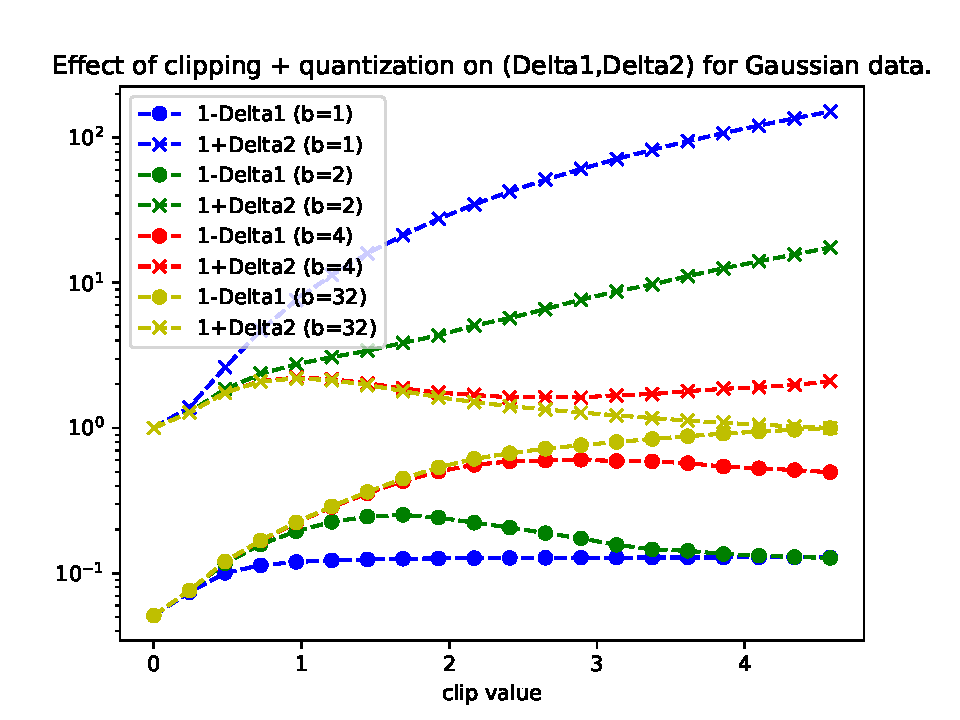
\includegraphics[width=0.8\columnwidth]{figures/deltas_vs_clip_and_quant.pdf}}
%		\caption{On random Gaussian data $X \in \RR^{1000\times 30}$, we demonstrate the joint effect of clipping and quantizing on $\Delta_1$ and $\Delta_2$, where we take $\lambda = \sigma_{\min}(X^T X)/10$.
%		A large clipping value gives large $\Delta_2$, whereas a small clipping values gives large $\Delta_1$.
%		This reveals the importance of choosing a clipping value which balances these two considerations.
%		}
%		\label{fig:deltas_vs_clip_quant}
%	\end{center}
%\end{figure}
